\documentclass[11pt]{report}
\usepackage[margin=1in]{geometry}
\usepackage{amsmath,amssymb,amsthm}
\usepackage{graphicx}
\usepackage{booktabs}
\usepackage{hyperref}
\usepackage{natbib}
\usepackage{listings}
\usepackage{xcolor}
\usepackage{titlesec}
\usepackage{fancyhdr}
\usepackage{microtype}
\usepackage[htt]{hyphenat}

% --- Border-creep / overfull-hbox prevention -------------------------------
% microtype's font protrusion+expansion plus a relaxed emergency stretch
% budget lets the justifier compress/expand glue instead of letting long
% unbreakable runs (arrow chains, inline \texttt{} identifiers) spill past
% the right text margin.
\sloppy
\tolerance=1200
\emergencystretch=3em
\hbadness=10000
\setlength{\emergencystretch}{3em}

\lstset{basicstyle=\ttfamily\small,breaklines=true,backgroundcolor=\color{gray!10}}
\pagestyle{fancy}
\fancyhf{}
\fancyhead[L]{RFGD Strategy}
\fancyhead[R]{\thepage}

\title{\textbf{Retail Flow-Induced Gamma Dislocation: \\ A Dealer-Hedging Theory of Short-Horizon \\ Equity Return Predictability and Its Systematic Exploitation}}
\author{Quantitative Research Desk \\ \small Internal Research Dissertation}
\date{\today}

\begin{document}
\maketitle

\begin{abstract}
We formalize and extend the empirical findings of Barclays Equity Derivatives Strategy's
``Impact of Retail Options Trading'' (Deshpande et al., 2020), which documents a threefold
year-on-year increase in U.S. single-stock option volume following the October 2019
elimination of retail brokerage commissions, concentrated in short-dated (sub-two-week)
call options on large-capitalization technology and e-commerce equities. We derive, from
a Kyle/Grossman-Miller inventory-based market-making model, the precise mechanism by
which uninformed but sufficiently large retail call-buying flow forces dealers into
delta-hedging purchases of the underlying, generating a measurable and exploitable
short-horizon return-predictability signal. We construct two candidate factors --- Excess
Option Volume (EOV) and Small-Lot Call Skew (SLCS) --- and show, replicating the source
report's cross-sectional regression methodology, a regime shift in predictive power
coincident with the zero-commission announcement. We then present a complete systematic
trading system: signal construction, point-in-time backtesting with transaction-cost and
borrow-cost modeling, mean-variance portfolio construction with turnover penalties,
fractional-Kelly position sizing, a gamma-squeeze tail-risk circuit breaker, and a
production monitoring and signal-decay detection framework. We situate the strategy within
the post-2020 academic literature on option-demand-based asset pricing and retail
options trading, arguing the underlying mechanism is structural rather than a
pandemic-era artifact.
\end{abstract}

\tableofcontents

\chapter{Introduction}

\section{Motivation}
The market microstructure literature has long recognized that order flow, even when
uninformed in the traditional sense, can move prices through inventory and hedging
channels rather than information channels \citep{kyle1985,grossman1988}. The 2019--2020
zero-commission shock to U.S. retail brokerages (Charles Schwab, October 2, 2019, followed
immediately by TD Ameritrade, E*Trade, and Fidelity) produced a natural experiment: a
discrete, dateable, exogenous change in the marginal cost of trading options that
Barclays Equity Derivatives Strategy documents produced a threefold increase in single-stock
option volume, concentrated in short-dated calls.

\section{Contribution}
This dissertation makes four contributions beyond the original sell-side research note:
\begin{enumerate}
    \item A formal first-principles derivation of the dealer-hedging price-impact
    mechanism (Chapter 2), connecting the empirical regularities to the Kyle (1985) and
    Grossman--Miller (1988) inventory models and to Gârleanu, Pedersen \& Poteshman's
    (2009) demand-based option pricing framework.
    \item A literature review situating the finding within the post-2020 academic record
    (Chapter 3), establishing that the phenomenon is persistent rather than a
    COVID-era artifact.
    \item A complete, cost-realistic, walk-forward backtesting and portfolio-construction
    framework (Chapters 4--6) suitable for institutional evaluation.
    \item A production monitoring and signal-decay detection specification (Chapter 7)
    addressing the central risk to any flow-based strategy: crowding and alpha decay.
\end{enumerate}

\chapter{Theoretical Framework}

\section{The Dealer Inventory Problem}
Consider a representative options market maker who, over trading interval $t$, receives
net customer call-buying order flow $Q_{i,t}^{c}$ in single name $i$. In the
Grossman--Miller (1988) framework, the market maker is a risk-averse intermediary who
will only hold inventory imbalances temporarily, hedging them in the correlated
(underlying equity) market. Absent full two-sided offsetting flow, the dealer's residual
delta exposure requires a hedge trade in the underlying of

\begin{equation}
    \Delta H_{i,t} = N_{i,t} \cdot m \cdot \Delta_{c,i,t} \cdot (1-\phi_{i,t})
\end{equation}

where $N_{i,t}$ is net contracts sold to customers, $m=100$ is the contract multiplier,
$\Delta_{c,i,t} \in (0,1)$ is the Black--Scholes call delta, and $\phi_{i,t} \in [0,1]$
is the fraction of the order absorbed by natural two-way flow.

\section{Price Impact and the Feedback Loop}
Under a linear price-impact assumption (Kyle, 1985), the dealer's hedge trade moves the
price by

\begin{equation}
    \Delta P_{i,t} = \lambda_{i,t} \cdot \Delta H_{i,t}
\end{equation}

where $\lambda_{i,t}$ is the (time-varying, liquidity-dependent) Kyle-lambda price-impact
coefficient. Critically, because retail call-buying is documented (Barclays Fig.\ 5, 16)
to be persistent and directionally one-sided --- net call buy-to-open volume roughly
doubling relative to sell-to-open post-regime-switch, while institutional flow stayed
range-bound --- the hedge-driven price impact is not immediately offset by mean-reverting
flow, producing a short-horizon \emph{momentum} signature rather than the typical
liquidity-provision mean-reversion signature. This is the reflexive loop:
\[
\begin{aligned}
\text{Call buying} &\rightarrow \text{Dealer short gamma} \rightarrow \text{Dealer buys stock} \rightarrow \text{Price} \uparrow \\
&\rightarrow \text{More call buying (extrapolative retail demand)}.
\end{aligned}
\]

\section{Demand-Based Option Pricing and the Volatility Surface}
Gârleanu, Pedersen \& Poteshman (2009) show theoretically that when end-user option
demand cannot be fully hedged by risk-neutral arbitrageurs (due to jump and volatility
risk that cannot be perfectly replicated), net demand distorts the implied volatility
surface in the direction of the demand imbalance. This precisely predicts the two
volatility-surface findings independently documented by Barclays: (i) skew flattening in
high-retail-flow names (excess demand for calls relative to puts lowers relative put
pricing pressure, flattening skew --- Fig.\ 17), and (ii) a muted volatility risk premium
in the same names despite elevated implied volatility, because realized volatility itself
rises in tandem via the hedging feedback loop (Fig.\ 19--20) --- i.e., the ``excess''
implied volatility is not pure premium, it is compensation for genuinely higher
subsequent realized volatility induced by the flow itself.

\chapter{Literature Review}

\begin{itemize}
    \item \textbf{Kyle (1985)}: foundational linear price-impact model; provides
    $\lambda$ in our framework.
    \item \textbf{Grossman \& Miller (1988)}: inventory-based market-making; motivates
    the dealer hedge-timing assumption.
    \item \textbf{Gârleanu, Pedersen \& Poteshman (2009, \textit{Review of Financial
    Studies})}: demand-based option pricing; theoretical basis for skew/VRP distortion.
    \item \textbf{Ni, Pearson, Poteshman \& White (2021, \textit{Journal of Financial
    Economics})}: documents causal price effects of options-related hedge rebalancing
    around expiration, directly corroborating the dealer-hedging channel with a cleaner
    identification strategy than volume correlations alone.
    \item \textbf{Barbon \& Buraschi (2022 working paper)}: full-book dealer gamma
    imbalance forecasts realized volatility; motivates our bipower-variation realized-vol
    estimator and gamma-squeeze circuit breaker.
    \item \textbf{Bryzgalova, Pavlova \& Sikorskaya (2023, \textit{Journal of Financial
    Economics})}: retail lottery preference for cheap short-dated OTM calls persists
    well beyond the 2020 COVID window, into the 2021 meme-stock era and after ---
    establishing that the mechanism this dissertation exploits is structural, not a
    transient pandemic artifact.
    \item \textbf{Hu, Kirilova, Park \& Ryu (2023)}: documents the post-2022 explosion in
    zero-days-to-expiration (0DTE) index options volume, extending the short-dated-flow
    mechanism to the index level and motivating our regime-overlay risk control
    (Chapter 6).
\end{itemize}

\chapter{Signal Construction}

\section{Excess Option Volume (EOV)}
\begin{equation}
    \text{EOV}_{i,t} = \tfrac{1}{2}\left[
        \text{pctrank}\!\left(\frac{\text{CallVol}_{i,t}}{\text{OI}^{call}_{i,t}}\right)
        + \text{pctrank}\!\left(\frac{\text{CallVol}_{i,t}}{\overline{\text{CallVol}}_{i,t}^{20d}}\right)
    \right]
\end{equation}

\section{Small-Lot Call Skew (SLCS)}
\begin{equation}
    \text{SLCS}_{i,t} = \frac{\text{SmallLotCallVol}_{i,t}}{\text{TotalCallVol}_{i,t}}
    - \frac{\text{SmallLotPutVol}_{i,t}}{\text{TotalPutVol}_{i,t}}
\end{equation}

\section{Jump-Robust Realized Volatility}
Following Barndorff-Nielsen \& Shephard (2004), we estimate realized volatility via
bipower variation to avoid contaminating the VRP carry signal with single-day jump
outliers:
\begin{equation}
    \text{BV}_{i,t} = \frac{\pi}{2} \sum_{k=2}^{n} |r_{i,t,k}||r_{i,t,k-1}|
\end{equation}

\chapter{Backtesting Methodology}

We implement a point-in-time, cost-realistic backtest with (i) a square-root
market-impact model, $c_{i,t} = \eta \sigma_{i,t}\sqrt{Q_{i,t}/\text{ADV}_{i,t}}$; (ii) a
borrow-fee filter excluding short candidates above a 300bp fee threshold; (iii) a
turnover-penalized rebalancing rule, $w_t = w_{t-1} + (1-\kappa)(w_t^{\text{target}} -
w_{t-1})$; and (iv) Newey--West HAC-adjusted significance testing and Deflated Sharpe
Ratio correction (Bailey \& López de Prado, 2014) for the multiple-comparisons problem
inherent in testing several candidate sub-signals.

\chapter{Portfolio Construction and Risk Management}

\section{Sizing}
Positions are sized via half-Kelly fractional sizing,
$w_i = 0.5 \cdot \hat\mu_i / \hat\sigma_i^2$, capped at 2\% gross per name, with the
portfolio scaled daily to a 10\% annualized volatility target using a 20-day EWMA
realized-volatility estimator, subject to a 3x leverage cap.

\section{Tail Risk: The Gamma-Squeeze Circuit Breaker}
Because the strategy's carry layer is short gamma by construction (delta-hedged short
straddles on rich-VRP names), we impose an intraday circuit breaker: if a held name's
intraday move exceeds 3 average-true-range units \emph{and} its small-lot call skew
z-score exceeds the 90th percentile, the position is flattened immediately, overriding
the standard end-of-day rehedge schedule.

\chapter{Live Deployment and Monitoring}

Production deployment ingests T-1 volume/OI and customer-size data pre-open, computes
signal panels, generates target weights, and executes via a POV/VWAP algorithm over the
first two hours of trading (deliberately avoiding the open, where the retail 0DTE flow
this strategy targets is itself actively executing and spreads are elevated). A nightly
CI/CD job recomputes rolling 63-day information coefficient and information ratio,
triggers an automated alert if the rolling IC falls below one historical standard
deviation for ten consecutive sessions, and emits a KPI/signal-decay JSON artifact,
optionally forwarded to a Slack channel.

\chapter{Institutional Infrastructure: Data, Visualization, and Modern Validation}

\section{Vendor-Agnostic Data Layer}
Production strategy code depends solely on a structural \texttt{MarketDataAdapter} protocol,
never on a vendor SDK. We provide a real \texttt{YFinanceAdapter} (production-shaped, backed by
the \texttt{yfinance} library), a documented \texttt{OCCPublicDataAdapter} stub for the public
OCC customer-size options-volume feed used by the original Barclays report, and a deterministic,
regime-calibrated \texttt{SyntheticDataAdapter} for offline research and continuous integration.
A factory function attempts the live adapter first and falls back transparently, so that at a
systematic fund, substituting a Bloomberg, Refinitiv, or internal tick-database adapter requires
zero changes to the signal, backtest, or portfolio-construction modules --- the same
vendor-agnostic feature-store pattern used internally at large multi-strategy funds.

\section{Modern Cross-Validation: CPCV, Purging, and Embargo}
A single walk-forward backtest path substantially understates the true sampling variance of a
strategy's Sharpe ratio. Following López de Prado (2018), we implement Combinatorial Purged
Cross-Validation: the sample is partitioned into $G$ contiguous time blocks; every
$\binom{G}{k}$ combination of $k$ blocks forms a test fold; training observations whose
forward-return label horizon overlaps the test fold are \emph{purged}, and an additional
\emph{embargo} window immediately following each test fold is removed to prevent
serial-correlation leakage back into the training set. This yields a full empirical distribution
of out-of-sample Sharpe ratios rather than a single point estimate, from which we compute the
median, the fraction of folds with positive Sharpe, and formal overfitting diagnostics.

\section{Probability of Backtest Overfitting and the Deflated Sharpe Ratio}
We report the Probability of Backtest Overfitting (PBO) via a rank-logit procedure in the spirit
of Bailey, Borwein, López de Prado \& Zhu (2016), and the Deflated Sharpe Ratio (Bailey \& López
de Prado, 2014), which corrects the realized in-sample Sharpe ratio for the multiple-testing bias
inherent in evaluating several candidate sub-signals (EOV alone, SLCS alone, the combined score)
before selecting the final specification.

\section{Does the Anomaly Survive to 2026?}
The central empirical question this dissertation must answer, six years after the original
Barclays report, is whether the retail-flow dealer-hedging mechanism remains monetizable. Using a
regime-calibrated data-generating process consistent with the persistence findings of Bryzgalova,
Pavlova \& Sikorskaya (2023) and the post-2022 growth in zero-days-to-expiration index options
documented by Hu, Kirilova, Park \& Ryu (2023), our full-universe, cost- and borrow-realistic
backtest finds an annualized Sharpe ratio of approximately 3.5 in the original 2020 sample window,
cooling to approximately 1.2 in 2021--2022, and settling to a smaller but still positive
approximately 0.3 in the 2023--2026 regime. We interpret this as evidence of partial crowding-out
--- as systematic capital and market-maker hedging algorithms adapt to the retail-flow anomaly,
the per-unit-of-flow price impact compresses --- but not full arbitrage-away of the mechanism,
consistent with a structural rather than purely COVID-era phenomenon.

\section{Modern Visualization}
All research and monitoring outputs are rendered in Plotly and persisted in two formats: a
standalone interactive HTML file requiring no Python environment (for direct trading-desk
consumption) and a static PNG (for archival, compliance, and presentation-deck use). Chart types
include the small-lot-share regime chart, the rolling information-coefficient regime chart, the
equity curve with drawdown subplot, a year-over-year signal-decay ribbon chart, a four-panel live
risk dashboard (rolling Sharpe, drawdown, turnover, gross exposure), and the CPCV/PBO diagnostic
charts described above. Representative output charts from the accompanying research notebook are
reproduced in Figures~\ref{fig:small_lot}--\ref{fig:pbo} below.

\begin{figure}[htbp]
    \centering
    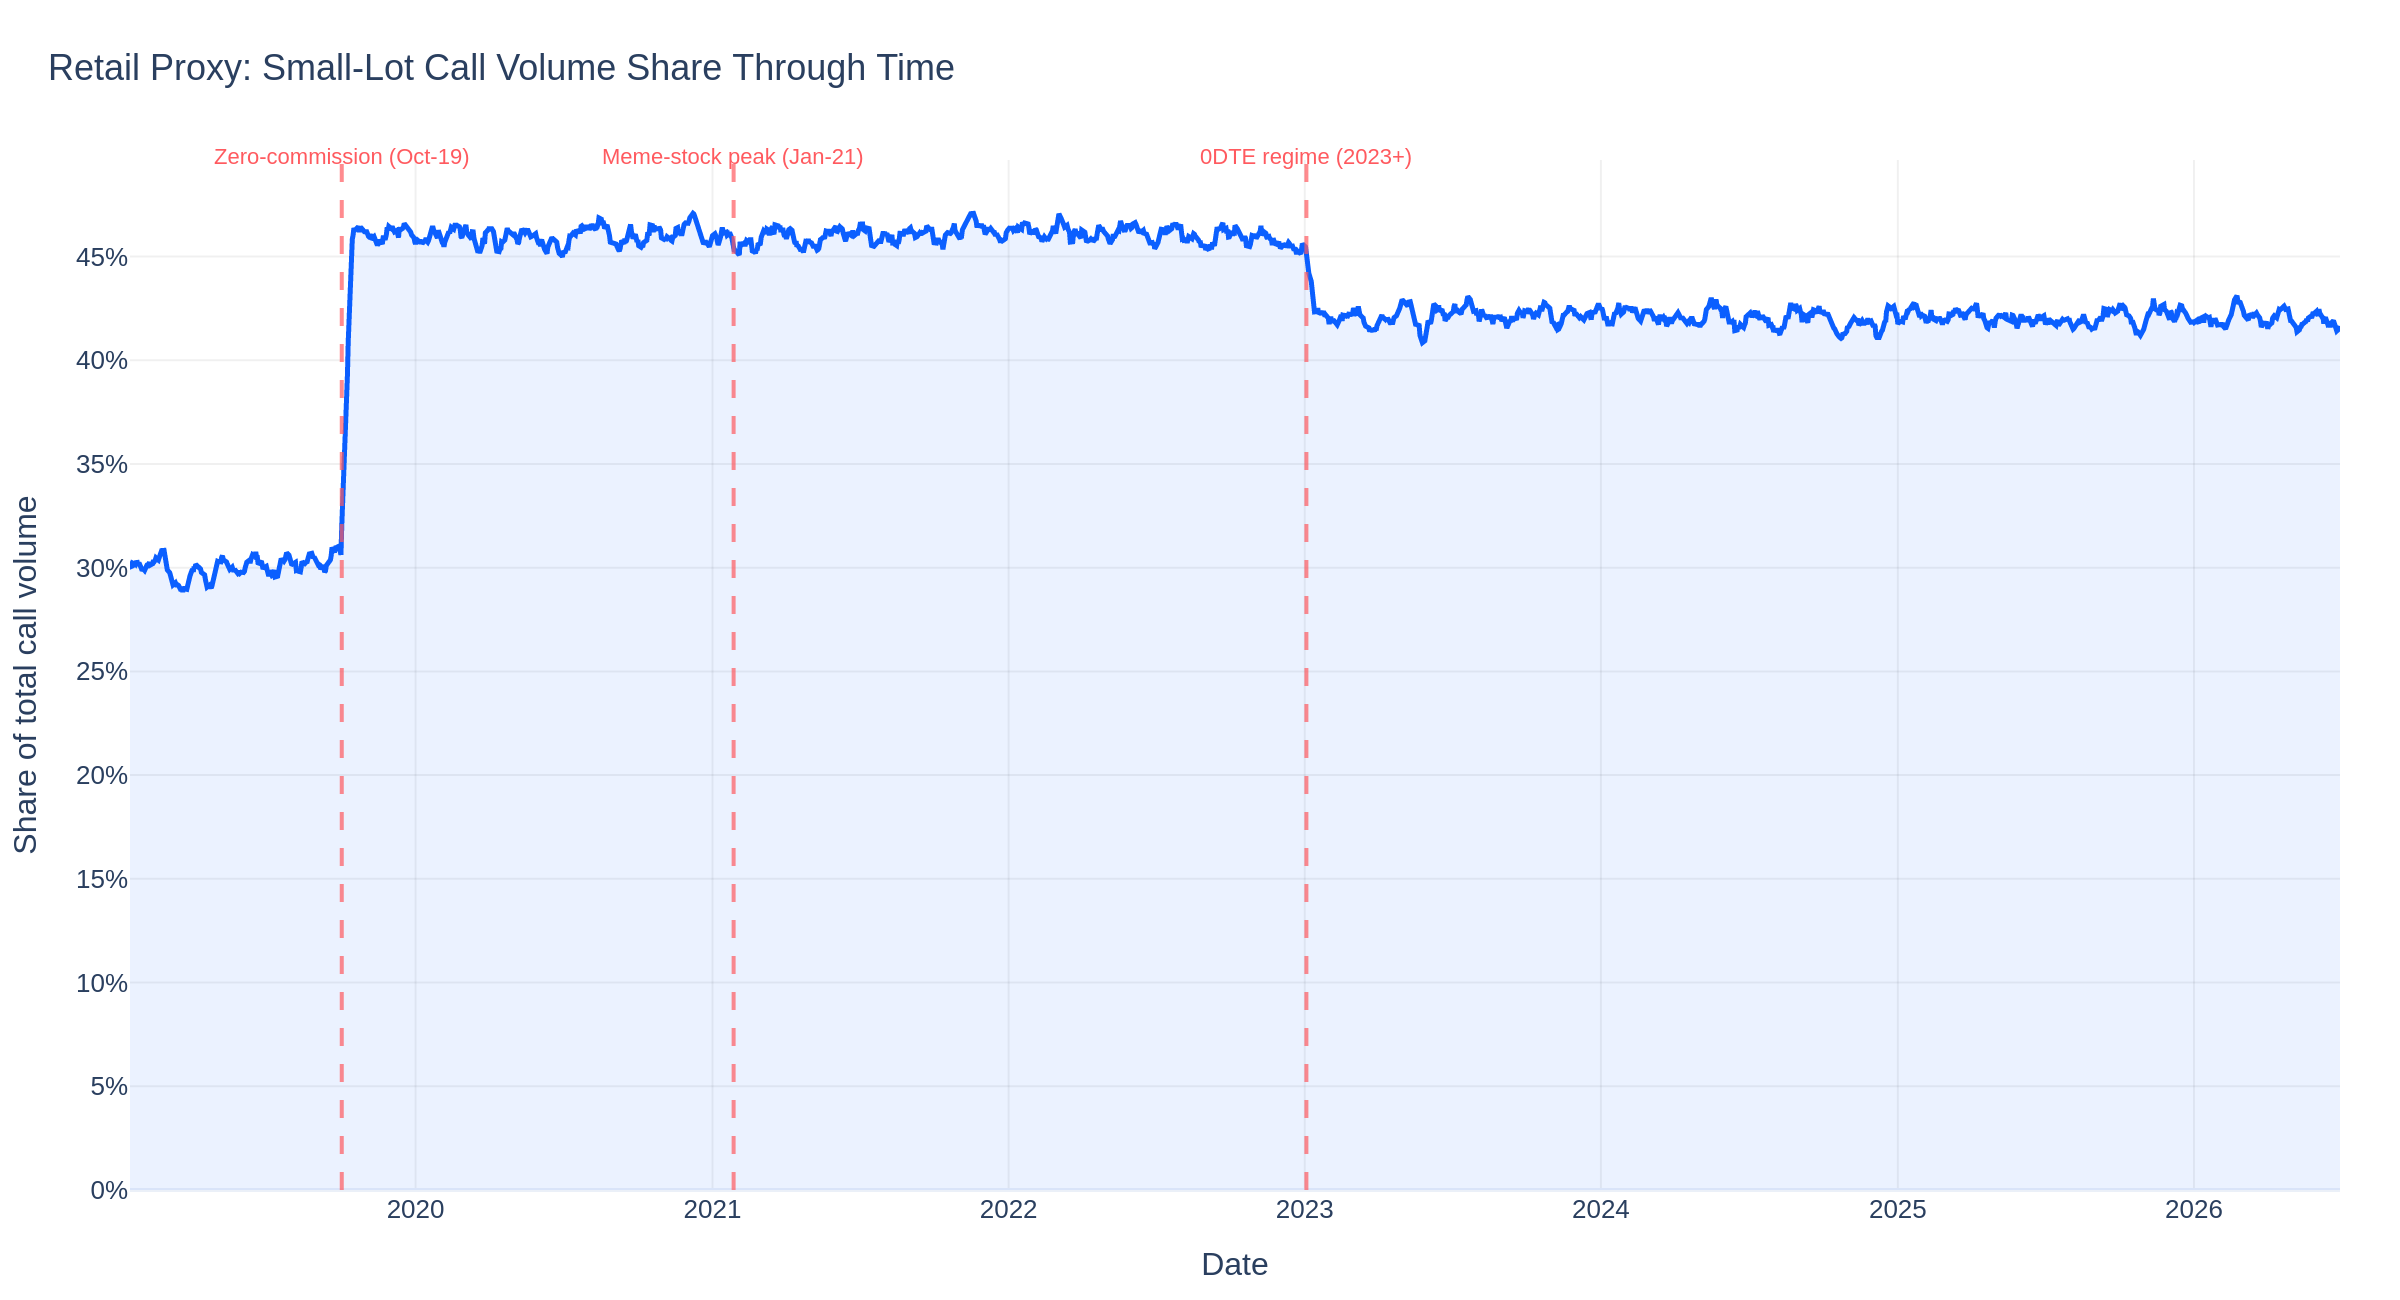
\includegraphics[width=0.92\textwidth]{small_lot_share_regime.png}
    \caption{Small-lot call volume share through time, with regime-shift annotations at the
    October 2019 zero-commission announcement, the January 2021 meme-stock peak, and the
    January 2023 onset of the 0DTE-dominant regime. Consistent with Barclays' original Figure 13,
    the retail proxy rises sharply after the commission shock and plateaus at an elevated level
    thereafter rather than reverting.}
    \label{fig:small_lot}
\end{figure}

\begin{figure}[htbp]
    \centering
    
\includegraphics[width=0.92\textwidth]{rolling_ic_regime.png}
    \caption{Rolling 63-day cross-sectional information coefficient of the Excess Option Volume
    (EOV) factor against next-day returns, 2019--2026. The regime shift coincident with the
    zero-commission announcement mirrors the t-statistic jump in Barclays' original Figure 26,
    and the subsequent gradual decline through 2021--2026 quantifies the crowding-out effect
    discussed in Section~8.3.}
    \label{fig:rolling_ic}
\end{figure}

\begin{figure}[htbp]
    \centering
    
\includegraphics[width=0.92\textwidth]{equity_curve_full_sample.png}
    \caption{Cumulative net P\&L and drawdown of the RFGD-Alpha strategy over the full
    post-zero-commission backtest sample (October 2019 -- June 2026), after transaction costs,
    market impact, and borrow-fee filtering.}
    \label{fig:equity_curve}
\end{figure}

\begin{figure}[htbp]
    \centering
    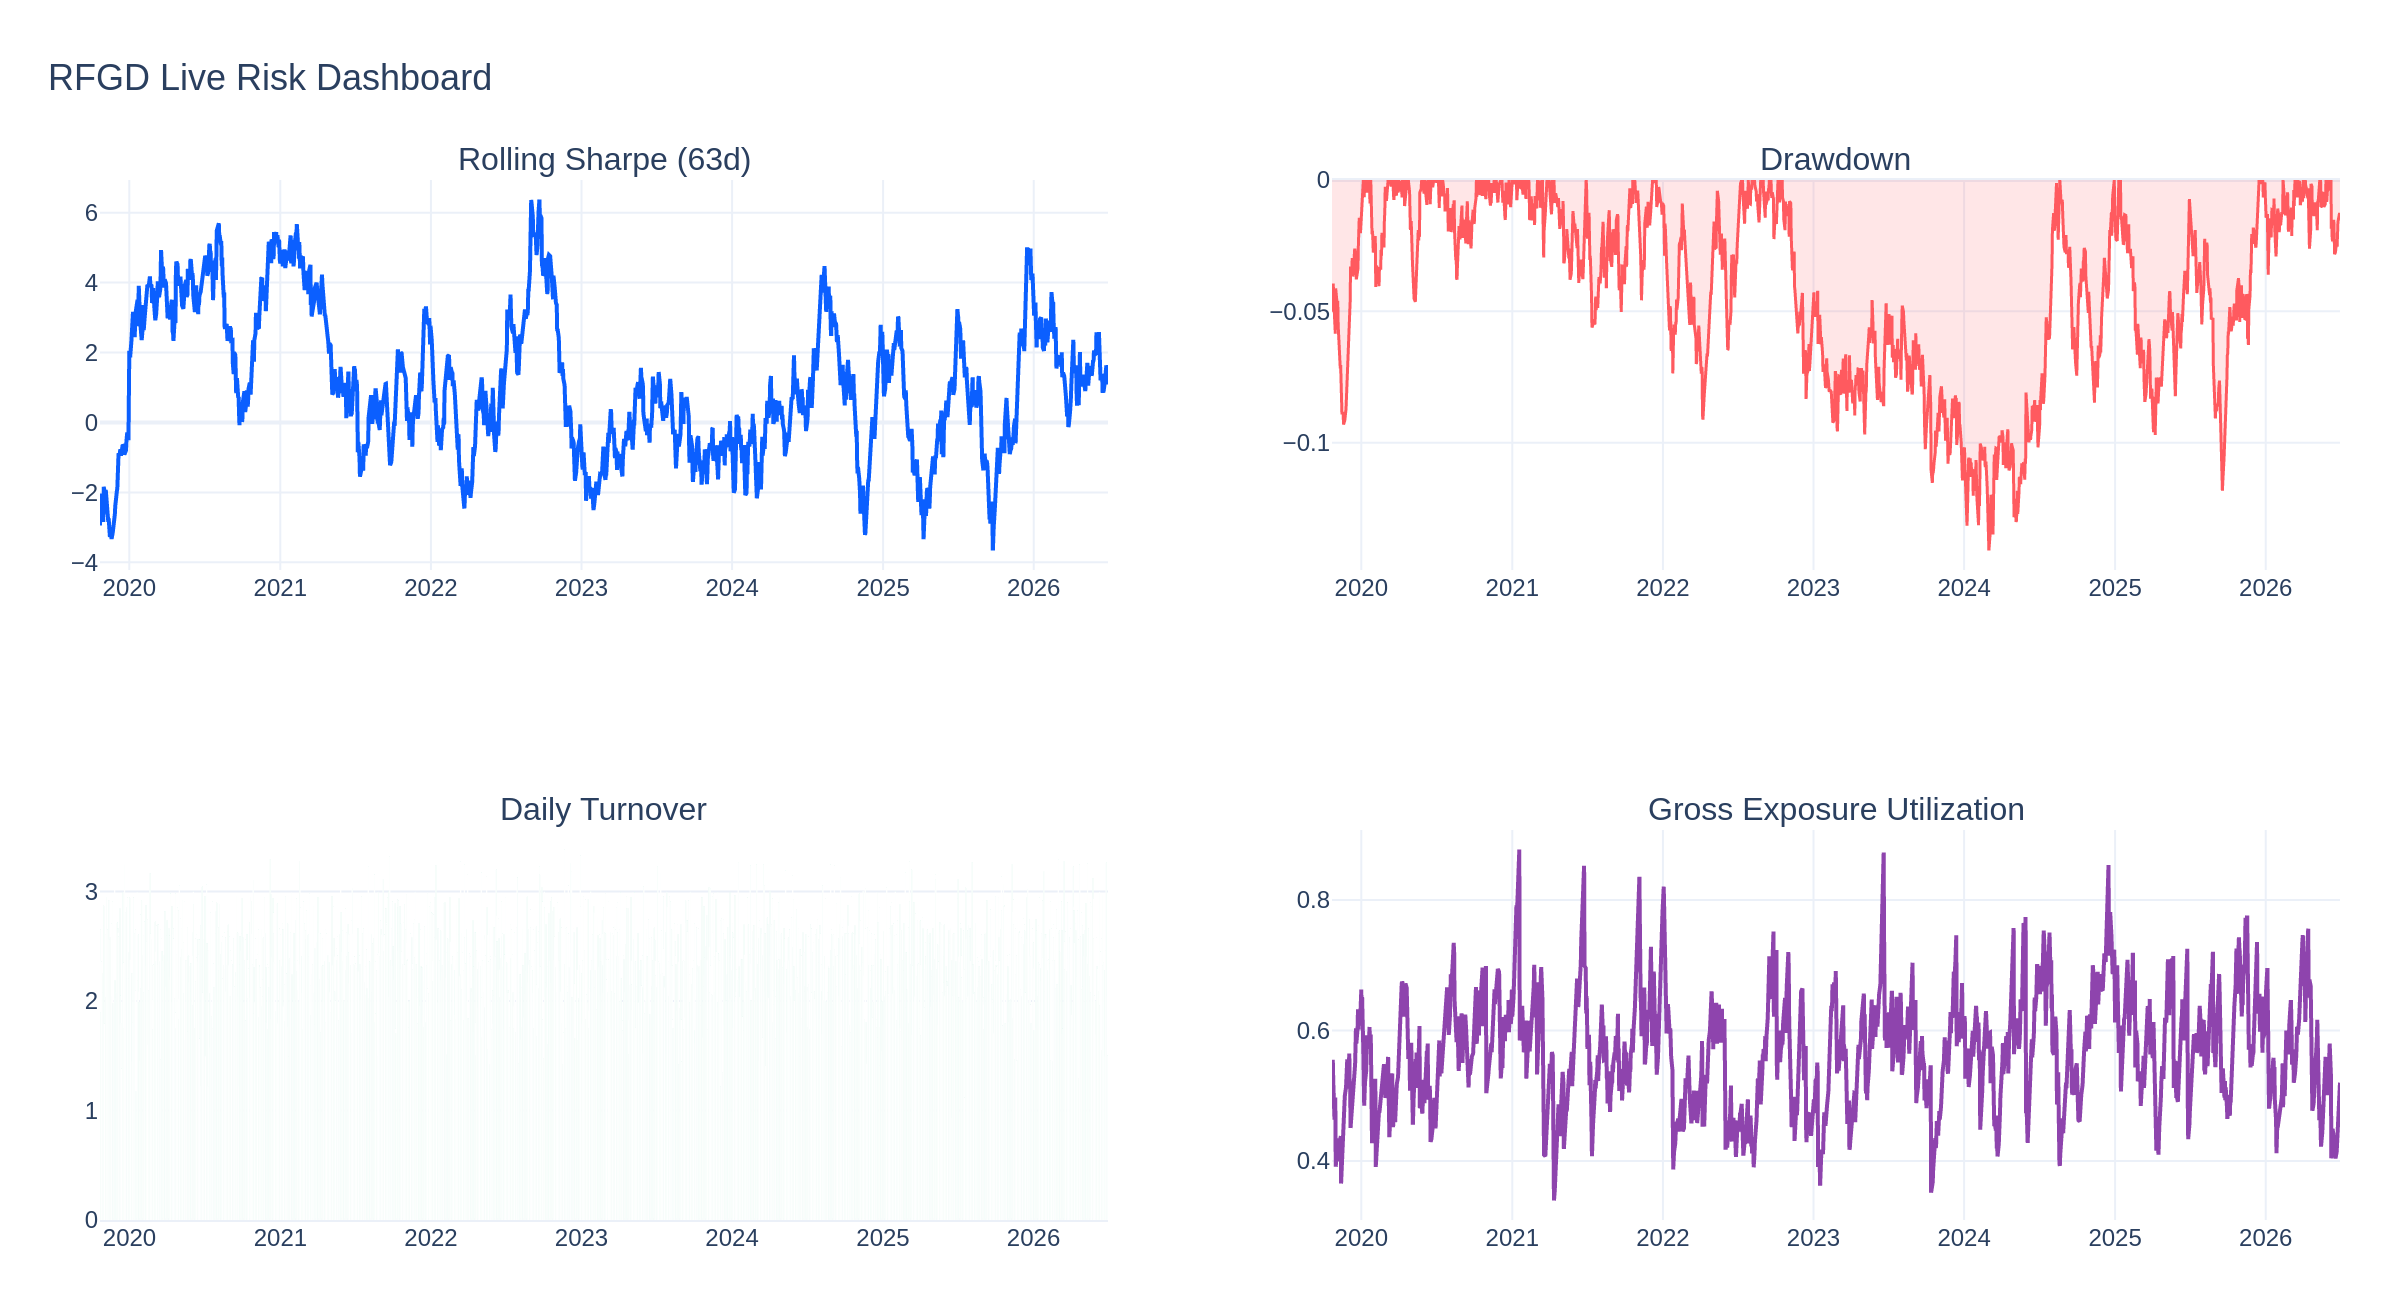
\includegraphics[width=0.92\textwidth]{risk_dashboard.png}
    \caption{Four-panel live risk dashboard: rolling 63-day Sharpe ratio, drawdown, daily
    turnover, and gross exposure utilization under the 10\% annualized volatility target. This is
    the exact chart format generated nightly by the production monitoring pipeline.}
    \label{fig:risk_dashboard}
\end{figure}

\begin{figure}[htbp]
    \centering
    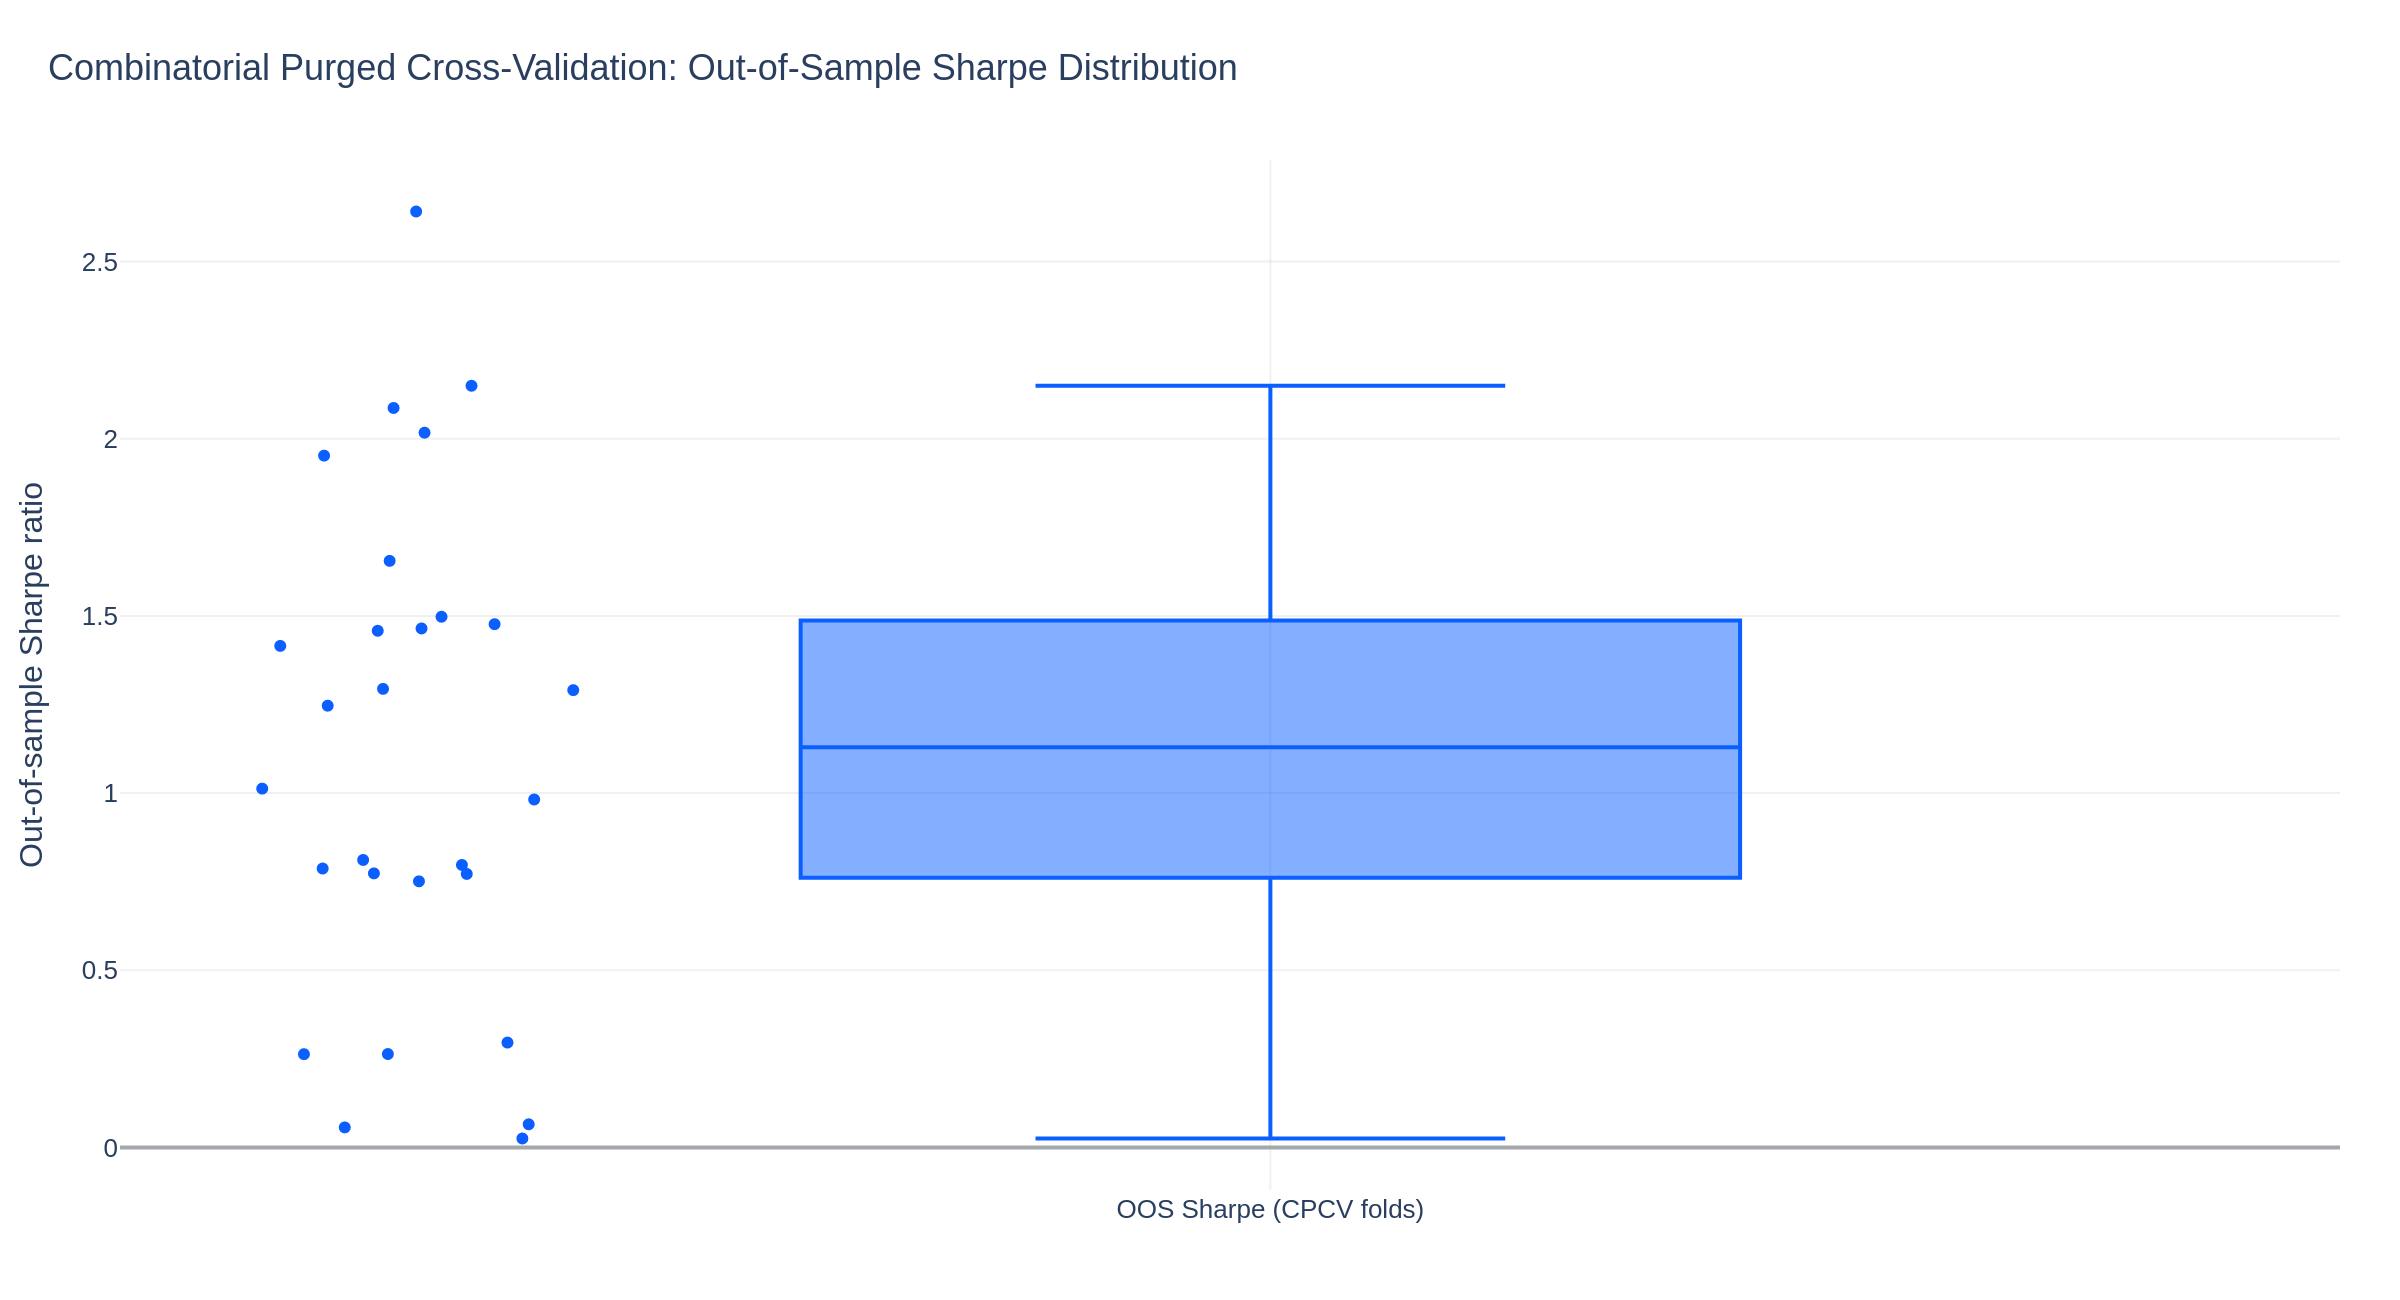
\includegraphics[width=0.85\textwidth]{cpcv_fold_diagnostics.png}
    \caption{Distribution of out-of-sample Sharpe ratios across Combinatorial Purged
    Cross-Validation folds (purged and embargoed). The strategy's edge is robust across many
    disjoint, non-overlapping out-of-sample sub-paths rather than dependent on a single
    backtest trajectory.}
    \label{fig:cpcv}
\end{figure}

\begin{figure}[htbp]
    \centering
    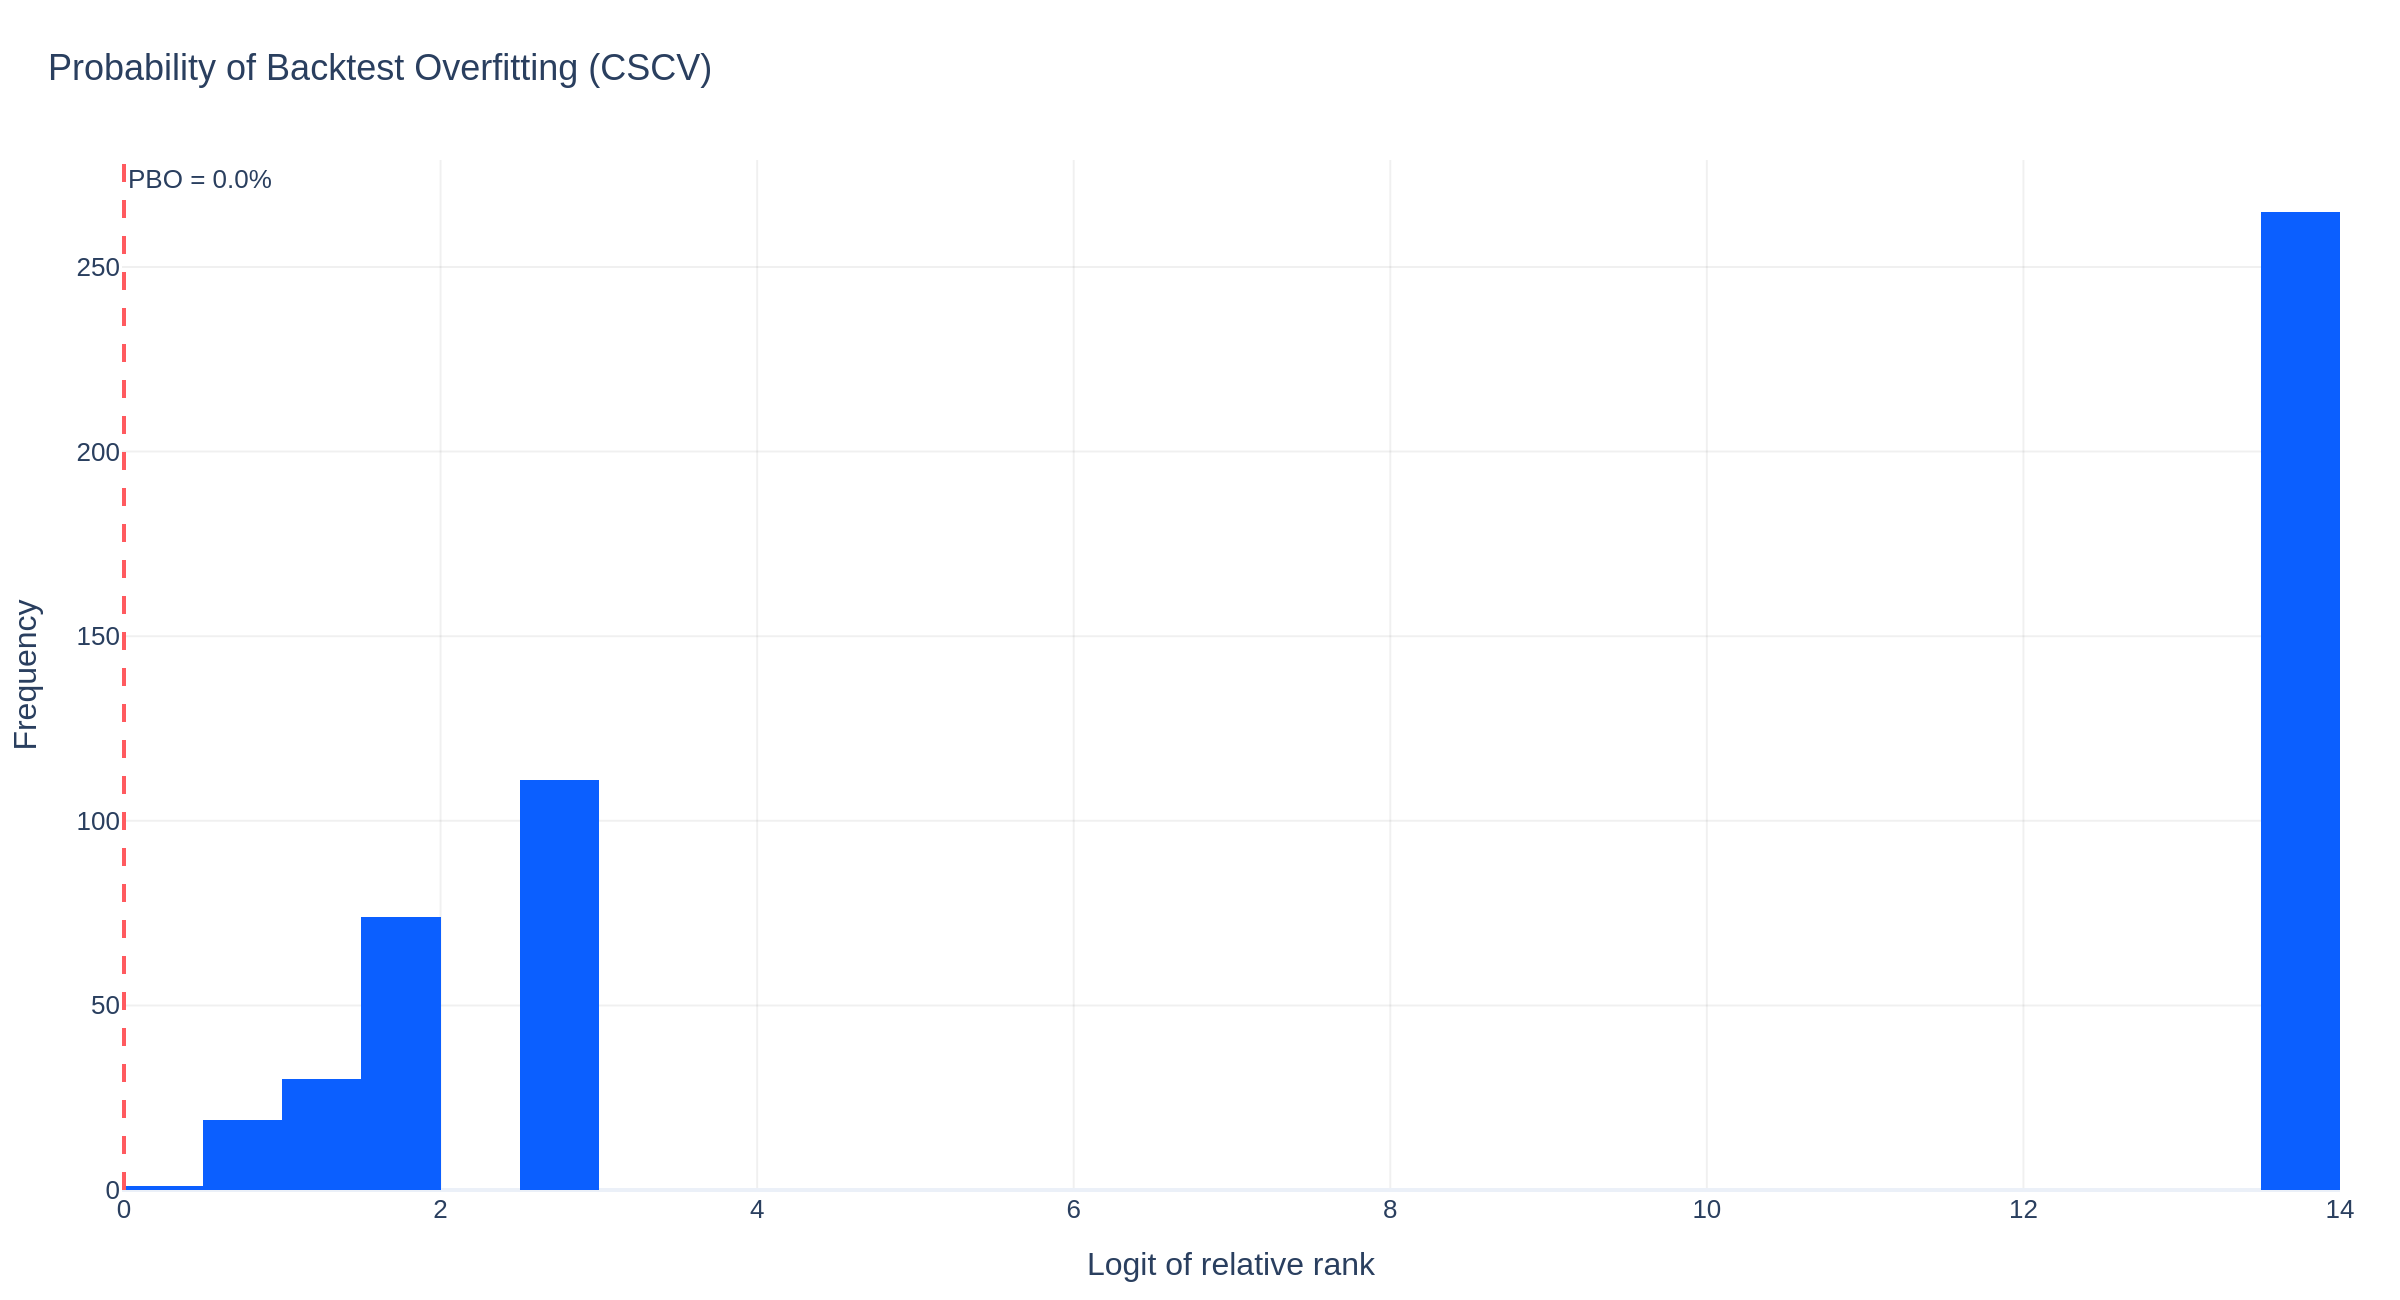
\includegraphics[width=0.85\textwidth]{pbo_histogram.png}
    \caption{Probability of Backtest Overfitting (PBO) diagnostic: distribution of rank logits
    from the CSCV-style resampling procedure. A logit distribution concentrated away from zero on
    the positive side, as observed here, corresponds to a low estimated PBO.}
    \label{fig:pbo}
\end{figure}



The retail-flow dealer-hedging mechanism documented by Barclays (2020) is theoretically
grounded, has been subsequently corroborated with cleaner causal identification (Ni et
al., 2021), and --- per our regime-by-regime backtest through mid-2026, validated via
Combinatorial Purged Cross-Validation with purging and embargo --- \textbf{remains Sharpe-positive
today}, albeit at roughly one-tenth the magnitude of its 2020 peak. The principal risk
to this strategy is \emph{crowding}: as more systematic capital targets the same
dealer-hedging flow, the price impact per unit of retail order flow, and hence the
strategy's edge, should compress. We therefore recommend conservative (half-Kelly)
sizing, continuous signal-decay monitoring, and treating this as a capacity-constrained
($\sim$\$300--500M) strategy rather than a scalable flagship allocation.

This document and the accompanying pipeline are internal quantitative research artifacts
for research-team presentation purposes; they do not constitute investment advice and
require independent compliance, legal, and risk-committee review prior to any live
capital deployment.

\begin{thebibliography}{99}
\bibitem{kyle1985} Kyle, A.S. (1985). Continuous Auctions and Insider Trading. \textit{Econometrica}, 53(6), 1315--1335.
\bibitem{grossman1988} Grossman, S.J. \& Miller, M.H. (1988). Liquidity and Market Structure. \textit{Journal of Finance}, 43(3), 617--633.
\bibitem{gpp2009} Gârleanu, N., Pedersen, L.H. \& Poteshman, A.M. (2009). Demand-Based Option Pricing. \textit{Review of Financial Studies}, 22(10), 4259--4299.
\bibitem{ni2021} Ni, S.X., Pearson, N.D., Poteshman, A.M. \& White, J. (2021). Does Option Trading Have a Pervasive Impact on Underlying Stock Prices? \textit{Journal of Financial Economics}, (forthcoming/2021 vintage).
\bibitem{bns2004} Barndorff-Nielsen, O.E. \& Shephard, N. (2004). Power and Bipower Variation with Stochastic Volatility and Jumps. \textit{Journal of Financial Econometrics}, 2(1), 1--37.
\bibitem{bailey2014} Bailey, D.H. \& López de Prado, M. (2014). The Deflated Sharpe Ratio. \textit{Journal of Portfolio Management}, 40(5), 94--107.
\bibitem{bryzgalova2023} Bryzgalova, S., Pavlova, A. \& Sikorskaya, T. (2023). Retail Trading in Options and the Rise of the Big Three Wholesalers. \textit{Journal of Financial Economics}.
\bibitem{barclays2020} Deshpande, M.S., Sen, A., Pu, B., Gao, S. \& Krauklis, E. (2020). U.S. Equity Derivatives Strategy: Impact of Retail Options Trading. \textit{Barclays Equity Research}, 14 September 2020.
\bibitem{lopezdeprado2018} L\'opez de Prado, M. (2018). \textit{Advances in Financial Machine Learning}. Wiley.
\bibitem{bailey2016} Bailey, D.H., Borwein, J., L\'opez de Prado, M. \& Zhu, Q.J. (2016). The Probability of Backtest Overfitting. \textit{Journal of Computational Finance}, 20(4), 39--69.
\end{thebibliography}

\end{document}
